\chapter{System Design}
\label{cha:design}

An operational investigator needs access to enough information to explain
a failure, but that access should not give its conclusions authority to
change the environment. It must also expose how an answer was reached
without making the operator reconstruct the investigation from raw logs.
The central design problem is therefore to connect evidence collection,
diagnostic reasoning and operator decisions while keeping their
responsibilities distinct.

The proposed system separates the application being investigated from the
investigation workflow. A common evidence interface supports three
diagnostic strategies, while an independently controlled executor handles
approved changes. This chapter specifies the component boundaries, data
contracts, investigation process and remediation controls that realise
the requirements in Chapter~\ref{cha:requirements}.

\section{Architecture and Component Boundaries}
\label{sec:design:architecture}

The architecture contains three application responsibilities. The test API
receives the requests whose behaviour is investigated. The investigation
host manages the operator interface, diagnostic runs and their records.
The remediation executor applies a narrowly defined set of approved
changes. They belong to the same project, but the test API and executor
run separately from the investigation host. Consequently, an application
exception does not also remove the interface needed to diagnose it, and
the investigator does not inherit the executor's write permissions.

Figure~\ref{fig:design:architecture} shows the principal interactions.
The operator uses an authenticated web interface to submit an endpoint,
time interval and symptom description. The host validates this scope,
creates an investigation record and schedules the chosen strategy. A
strategy selects evidence tools and produces a structured diagnosis.
Only the agent strategies use the model adapter. The same evidence
gateway serves the rule-based procedure and both agent configurations.

\begin{figure}[htbp]
\centering
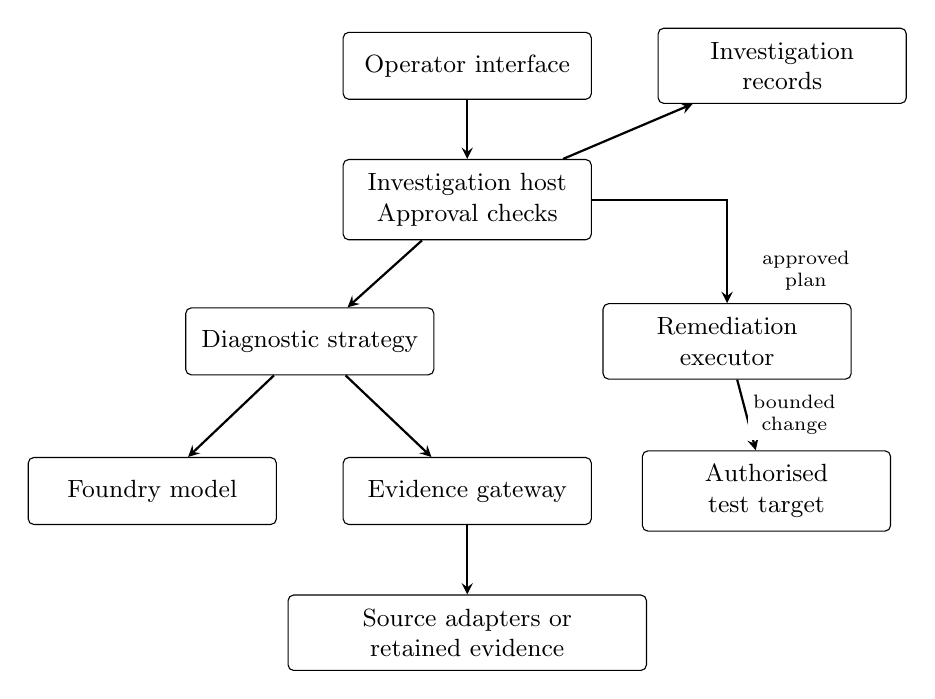
\begin{tikzpicture}[
  box/.style={draw, rounded corners=2pt, align=center, font=\small,
              text width=2.8cm, minimum height=0.85cm, inner sep=5pt},
  flow/.style={->, >=stealth, thick},
  note/.style={font=\scriptsize, fill=white, inner sep=2pt, align=center}]
\node[box] (ui) at (0,0) {Operator interface};
\node[box] (store) at (4,0) {Investigation records};
\node[box] (host) at (0,-1.7) {Investigation host\\Approval checks};
\node[box] (strategy) at (-2,-3.5) {Diagnostic strategy};
\node[box] (executor) at (3.3,-3.5) {Remediation executor};
\node[box] (model) at (-4,-5.4) {Foundry model};
\node[box] (gateway) at (0,-5.4) {Evidence gateway};
\node[box] (target) at (3.8,-5.4) {Authorised test target};
\node[box, text width=4.2cm] (sources) at (0,-7.2)
  {Source adapters or retained evidence};
\draw[flow] (ui) -- (host);
\draw[flow] (host) -- (store);
\draw[flow] (host) -- (strategy);
\draw[flow] (host.east) -| (executor.north);
\node[note] at (4.3,-2.6) {approved\\plan};
\draw[flow] (strategy) -- (model);
\draw[flow] (strategy) -- (gateway);
\draw[flow] (gateway) -- (sources);
\draw[flow] (executor) -- node[note, right] {bounded\\change} (target);
\end{tikzpicture}
\caption{Logical components and principal requests. Results return to the
caller. The record store also retains evidence and execution history.
The diagram describes software responsibilities, not the physical order
of network devices in the application request path.}
\label{fig:design:architecture}
\end{figure}

The four source adapters correspond to Cloudflare, Azure Firewall, Azure
infrastructure and application telemetry. They are logical interfaces,
not necessarily four different storage systems. For example, application
and firewall records can be obtained from the same Log Analytics workspace
while retaining different schemas and meanings. Prepared telemetry from
the wider observability platform is preferred. A direct source API is
used where the required observations are not available through that
platform, as permitted by the Norlys specification
\parencite[Relationship to the Parent Story, AC-3]{norlys_operations_agents}.
The OpenTelemetry collector transports telemetry. It neither hosts the
investigator nor decides which diagnosis is correct.

The investigation host uses explicit orchestration in C\# rather than
delegating the complete workflow to a managed agent runtime. This makes
tool dispatch, stopping conditions and resource accounting part of
inspectable application logic. Foundry supplies model inference through
an adapter. Agent roles are separate conversation contexts inside the
investigation process, rather than separately deployed services. This
retains the specification's coordinator-and-specialist organisation
without requiring a deployment for each role
\parencite[Architecture Sketch]{norlys_operations_agents}.

Within each service, controllers validate incoming requests, application
services implement use cases, and repositories handle external input and
output. Domain records represent evidence, diagnoses and plans without
depending on Azure or model-client types. An investigation service owns
the run loop and calls strategy components and repository interfaces.
Provider-specific responses are translated at the boundary. This permits
the model client or evidence source to change without changing the
diagnostic result expected by the interface and evaluator.

The browser communicates with the host over authenticated HTTPS using
JSON records. Starting an investigation returns its identifier and a
pending status, allowing the browser to retrieve progress without holding
one long request open. A background worker advances the run and persists
its state. Cancellation prevents new diagnostic calls. An interrupted run
is recorded as interrupted rather than silently restarted with a fresh
allowance. The initial PoC processes one investigation at a time, which
also avoids competition between comparison runs for model quota. The
executor exposes a separate authenticated interface accepting a plan
identifier, never an arbitrary command. Its own policy checks remain
necessary even when the request comes from the investigation host.

Azure Container Apps is the deployment target for the investigation host
and executor in the development landing zone. They reference the project's
existing infrastructure where suitable. Process separation protects
against faults confined to the test API, but not an outage of an entire
shared hosting environment. Experiments affecting that wider environment
therefore require the investigation controls to be hosted outside the
affected resource boundary. Shared production firewalls and tunnel
connectors remain observation sources, not change targets.

\section{Evidence Access and Data Contracts}
\label{sec:design:evidence}

\subsection{Bounded Tools and Explicit Query Outcomes}

The gateway exposes typed operations for retrieving requests, related
application logs, security events, infrastructure observations and
configuration context. An operation accepts an investigation identifier,
an allowed target, a time interval and supported filters. The host binds
the investigation's maximum scope before any model call. A strategy may
narrow that scope but cannot enlarge it by supplying another subscription,
hostname or destination.

Queries use parameterised templates with validated arguments. The model
does not receive a general Kusto query editor, arbitrary HTTP client or
shell. This reduces query flexibility, but makes source restrictions,
output limits and comparison conditions enforceable. New diagnostic
capabilities require an explicit tool definition that is available to
all compared strategies. Pagination uses stable ordering and bounded
pages, with each additional request charged to the tool allowance.

Table~\ref{tab:design:contracts} defines the shared records. An evidence
identifier refers to an observation retained by the system, rather than
text generated by an agent. Source-specific fields remain typed, so that
an HTTP response status cannot be confused with a firewall action.
Event time and retrieval time are separate. Ingestion time is retained
where the source exposes it.

\begin{table}[htbp]
\centering\small
\caption{Core records exchanged between components.}
\label{tab:design:contracts}
\begin{tabularx}{\textwidth}{@{}>{\raggedright\arraybackslash}p{0.22\textwidth}>{\raggedright\arraybackslash}X@{}}
\toprule
Record & Essential content \\
\midrule
Investigation & Identifier, endpoint, interval, reported symptom, expected behaviour, strategy, evidence mode and limits. \\
\addlinespace
Evidence item & Identifier, source, resource, event time, available correlation fields, typed observations and provenance. \\
\addlinespace
Query result & Status, applied scope, evidence references, coverage, truncation, continuation information and retrieval time. \\
\addlinespace
Path link & Related items or components, matching basis, supporting references and ambiguity or missing information. \\
\addlinespace
Diagnosis & Outcome, primary component and cause, claim-to-evidence links, alternatives, evidence gaps and uncertainty explanation. \\
\addlinespace
Run record & Configuration versions, tool and model calls, usage, final result and termination reason. \\
\bottomrule
\end{tabularx}
\end{table}

A query result distinguishes successful retrieval, no matches, partial
results, unavailable coverage, access denial and execution failure. A
successful query with zero rows means only that its filters returned no
observations. It does not establish that the source collected all relevant
events. Coverage information therefore records the source and interval
represented, known collection gaps and any sampling or truncation.
Unknown coverage remains unknown. Error details describe the failed
operation without exposing credentials or unrestricted source content.

The gateway applies resource and time filters before returning evidence.
Only an explicit set of fields enters the model context. Authentication
headers, cookies, secrets and unrelated payload content are excluded.
Where identifiers must be masked, the transformation preserves equality
within the investigation so that related records can still be matched.
Masking does not turn connection-level evidence into request-level
evidence. Workspace-level read permissions may still permit the service
identity to access more data than the gateway returns. Application filters
are therefore an additional boundary, not a claim of row-level Azure
authorisation.

\subsection{Live Retrieval and Retained Evidence}

The evidence interface has two implementations. Live adapters query the
operational sources. A retained-evidence adapter queries a fixed collection
using the same filters, schemas and result statuses. The mode is fixed
when a run starts. A missing observation in a retained collection cannot
trigger an unnoticed fallback to a live source.

A collection manifest records its scope, capture interval, source
coverage, schema and masking versions, and checksums of its contents.
Configuration observations include their observation time. Current
configuration cannot silently stand in for the configuration at an older
incident. Collections are assembled from scoped source records, rather
than only the records selected during a previous agent investigation.
This allows each strategy to choose its own queries over the same
available evidence, as required by
Section~\ref{sec:methodology:procedure}.

The three security-evidence views in
Section~\ref{sec:methodology:procedure} are enforced by a projection at
this boundary. The projection defines which fields and summaries each
tool can expose. It also applies to configuration context, record-detail
lookups and error messages. A removed rule field must not remain available
inside a raw log message or through an alternative query. Derived features
are computed only from the permitted view.

Protected JSON artefacts in private Azure Blob Storage are the proposed
persistence format for collections, transcripts and final outputs.
Small manifest records support listing and reopening investigations,
avoiding a separate analytical database for the PoC. Payloads are written
under new identifiers before a manifest references them. Finalised
artefacts are not overwritten through the application interface.
Checksums detect accidental changes but do not replace access control.
Mutable workflow records use conditional updates to prevent two
requests from overwriting the same state. Azure Blob Storage supports
this through entity tags, which identify the version read by a caller
\parencite{microsoft2026blobconcurrency}.

The evidence repository is separate from the evaluation reference store.
Fault labels, injection commands and expected answers are not present in
the investigator's container, configuration or storage permissions.
Retention and deletion apply to retained evidence as well as the original
monitoring data. Exporting a collection does not create permission to
retain it indefinitely.

\section{Correlation and Security Features}
\label{sec:design:correlation}

Correlation starts from a versioned description of the selected endpoint
and its relevant components. This description contains the hostname,
application target and permitted network relationships. It distinguishes
configuration knowledge from relationships supported by observations.
Seeing records from two firewalls does not, by itself, determine their
physical order or prove that they describe two separate HTTP requests.

The correlation component first groups observations with usable
identifiers. An application operation identifier connects the request
record with its related logs. A Cloudflare Ray ID recorded at the origin
can connect edge and application observations. Cloudflare documents both
its propagation in the \texttt{Cf-Ray} header and the possibility that
different requests share an identifier
\parencite{cloudflare2026rayid}. The design therefore checks the identifier
alongside time, hostname and available request details. It records the
matching basis instead of treating the identifier as an unconditional
uniqueness guarantee.

Where identifiers are absent, the component retrieves candidates using a
bounded time interval, connector address, destination, port and protocol.
The interval includes an explicitly configured tolerance for timing
differences. If several observations satisfy these conditions, all remain
candidates. The component does not select the nearest timestamp and label
it as the exact request. A path link is classified as
\emph{identifier-supported}, \emph{inferred}, \emph{ambiguous} or
\emph{unobserved}. Each link carries its evidence references and the
conditions used to create it. The investigator can interpret the links
but cannot strengthen their classification without additional evidence.

This produces a partial evidence graph: components and observations are
nodes, and supported or candidate relationships are edges. It is an
investigation artefact, not a complete network topology. The operator can
inspect a missing segment without the interface drawing a continuous
trace that the observations do not support. Correlation rules run outside
the model and are shared by the three strategies, isolating the value of
diagnostic reasoning from differences in basic record matching.

Security features retain the distinction between a request and a logged
network event. Table~\ref{tab:design:features} defines the initial feature
set. Each result includes its source, filters, interval and contributing
record identifiers. Repeated ingestion of the same identifiable record
is removed, but observations from different firewalls remain separate.
A logged record is not assumed to represent a unique connection unless
the source provides the fields needed to establish that.

\begin{table}[htbp]
\centering\small
\caption{Security evidence exposed by the gateway. Missing coverage is
reported separately from a measured zero.}
\label{tab:design:features}
\begin{tabularx}{\textwidth}{@{}>{\raggedright\arraybackslash}p{0.25\textwidth}>{\raggedright\arraybackslash}X@{}}
\toprule
Evidence or feature & Definition and interpretation \\
\midrule
Decision context & Recorded action, rule identifier, policy context and intended permission for the scoped traffic. A denial is not itself proof of misconfiguration. \\
\addlinespace
Denied-record count & Number of matching deny records, grouped by firewall, target and rule where available. It is not a count of failed HTTP requests. \\
\addlinespace
Denied-record fraction & Deny records divided by matching records with a known allow or deny action, within the same group. An empty denominator gives no value. \\
\addlinespace
Edge outcome counts & Cloudflare request records grouped by recorded action or response status for the selected hostname and interval. Sampling and absent fields remain visible. \\
\addlinespace
Temporal distribution & Counts in fixed-duration intervals, preserving the source and unit. These indicate when observations concentrate, without establishing causation. \\
\bottomrule
\end{tabularx}
\end{table}

The legitimate request's intended behaviour is supplied as operational
context to every strategy. It states, for example, which authenticated
test operation should be permitted. It does not state the injected fault.
This distinction allows an investigator to interpret a blocking decision
without receiving the reference answer. If the applied policy cannot be
read, the result can identify an observed denial but must leave unsupported
details about the erroneous rule unresolved.

\section{Investigation Strategies and Orchestration}
\label{sec:design:investigators}

\subsection{A Common Investigation Contract}

Each strategy receives the investigation record, the same operational
context and access to the evidence gateway. It returns one primary
diagnosis. The outcome is a diagnosed fault, no fault found within the
scope, or insufficient evidence. Run status is separate: a timeout or
invalid final response is an execution outcome, not a healthy diagnosis.

A diagnosis links its decisive claims to evidence identifiers. Alternatives
state what remains plausible and which observation would distinguish them.
Uncertainty is expressed through evidence gaps and the strength of the
supported conclusion. The design does not assign an uncalibrated numeric
probability to the model's confidence. Before accepting an output, the
host validates its schema, required fields, target scope and references.
These checks establish that the result is well formed and traceable.
They do not establish that its explanation is correct, which still
requires the assessment in Section~\ref{sec:methodology:measures}.

The rule-based strategy represents a troubleshooting procedure as explicit
conditions, evidence requests and stopping rules. A condition can be true,
false or unknown, allowing missing coverage to differ from an observed
absence. Branches request additional observations or produce a qualified
result. Rules may combine observations across sources and are not limited
to one fixed order. Every conclusion records the matched conditions and
their evidence. The reviewed rules and any repair templates are versioned
configuration. No rule reads the case identifier as a diagnostic label.

\subsection{Single and Collaborating Agents}

The single investigator runs a bounded interaction loop. The host supplies
the task, tool definitions and current context. The model returns a tool
request or a final diagnosis. For a tool request, the host validates the
operation and arguments, executes the permitted query and returns its
structured result. The model can then request more evidence or revise its
conclusion. The loop stops at a valid final output, cancellation, an
unrecoverable error or the first resource limit. A malformed call can be
returned as a validation error within the fixed retry allowance.

The collaborating configuration contains a coordinator and two
specialists. The network and security specialist examines Cloudflare,
firewall decisions and the observable connection path. The application
and platform specialist examines request failures, application logs,
hosting state and relevant configuration. Grouping these responsibilities
reduces hand-offs between tightly related sources while preserving
different diagnostic perspectives. Compared with one specialist per
source, it also leaves more of the common allowance for collecting and
interpreting evidence. Whether this organisation is beneficial remains
an experimental question.

The coordinator owns the investigation and the final result. It sends each
specialist a bounded question, relevant evidence references and the
remaining allowance. A specialist returns findings in a common format:
claim, supporting and conflicting evidence, missing observations and a
suggested next check. Findings enter a shared evidence ledger, while
conversation histories remain separate. The coordinator can request a
follow-up within the limits and must resolve or preserve disagreements.
Agreement by two agents is not added to the ledger as independent
observational evidence.

Specialisation changes instructions, not access rights. Every agent can
use the same underlying tools, and the single investigator receives the
same substantive diagnostic guidance. Specialist responses reference the
original observations so that the coordinator can inspect them directly.
The design avoids mandatory full transcripts between agents, which would
duplicate context and consume resources without necessarily adding
evidence. A deterministic scheduler services one outstanding model or
tool call at a time. This first configuration tests collaboration without
also introducing parallel execution as a source of latency differences.

\subsection{Limits and Failure Handling}

One run-level budget manager accounts for all calls, including specialist
requests, coordination, validation retries and final-answer generation.
Before a model call, it checks the input size and reserves an output
allowance from the remaining total. Actual usage is then reconciled with
the reservation. Reported reasoning tokens are included without being
counted twice. A provider error with unknown usage remains marked as
unknown rather than being recorded as a free call. Tool requests, including
failed attempts, consume the common tool allowance.

Time limits cancel further work and retain the last available evidence.
Any unfinished conclusion is labelled as such rather than promoted to a
valid diagnosis. Context reduction, if needed, follows the same explicit
policy in both agent configurations and preserves evidence identifiers
and query coverage. Repeated failure does not trigger a different model
or unrestricted tool. Such a fallback would change the method during its
evaluation. The run record retains requests, results, visible findings and
usage, without requiring access to private internal model reasoning.

\section{Model Integration and Data Protection}
\label{sec:design:model}

The model adapter targets a managed deployment in the project's Microsoft
Foundry resource. It translates domain messages and tool descriptions into
the provider's format and translates responses into tool requests or final
outputs. Microsoft documents Entra ID authentication and application-side
handling of function calls through the Responses API
\parencite{microsoft2026responses}. The model therefore proposes an
operation. The application remains responsible for deciding whether that
operation can run.

The initial integration candidate is \texttt{gpt-6-luna}, the lightweight
GPT deployment selected for the project. The previously considered
\texttt{claude-haiku-5-5} candidate requires tenant Marketplace approval,
which makes deployment eligibility
a practical distinction between the candidates. This is an access
constraint, not evidence that GPT provides better diagnoses. A larger
eligible model is relevant only if its development-case results justify
its additional resource use. Table~\ref{tab:design:model} sets out the
comparison that determines the fixed evaluation model.

\begin{table}[htbp]
\centering\small
\caption{Model-selection criteria and the evidence needed for a decision.}
\label{tab:design:model}
\begin{tabularx}{\textwidth}{@{}>{\raggedright\arraybackslash}p{0.27\textwidth}>{\raggedright\arraybackslash}X@{}}
\toprule
Criterion & Basis for selection \\
\midrule
Deployment eligibility & Available in the project landing zone with an acceptable processing boundary, access method and quota. \\
\addlinespace
Tool and output behaviour & Development tests of valid tool requests, structured diagnoses, reference preservation and failure handling. \\
\addlinespace
Diagnostic usefulness & Supported component and cause identification on the same development cases, including healthy and incomplete-evidence cases. \\
\addlinespace
Resource use & Measured latency, token usage and estimated cost under the same single-investigator workflow. \\
\addlinespace
Reproducibility & Identifiable model version and settings that can remain fixed throughout the reserved evaluation. \\
\bottomrule
\end{tabularx}
\end{table}

\thesisTODO{Complete the model comparison using the Chapter 5 pilot.
Record the eligible model names and versions, observed results and the
reason for the final selection. Connectivity alone does not complete
this comparison.}

Conversation state is managed by the application, with provider-side
response storage disabled where supported. This permits a fresh context
for each investigation and explicit control over what is retained locally.
Disabling response storage is not a general guarantee of zero service-side
retention \parencite{microsoft2026responses}. The Foundry resource's
location also does not establish the location of inference. Microsoft's
deployment documentation distinguishes global processing, processing
within a defined data zone and processing within an Azure geography
\parencite{microsoft2026foundrydeployments}. The permitted data boundary
must therefore be checked against the deployment type as well as the
resource location.

\thesisTODO{Confirm with Norlys which evidence fields may reach the model,
the permitted processing boundary, and access and retention rules for
investigation artefacts. Bind these decisions to the gateway's field
policy and the selected deployment configuration.}

Retrieved text is treated as untrusted data. A log message can contain
instructions, including content originating outside the application.
Greshake and colleagues demonstrate how instructions embedded in retrieved
content can redirect an LLM application's behaviour
\parencite{greshake2023indirect}. The design therefore separates tool
results from system instructions and validates every requested operation
outside the model. The diagnostic tool set contains no mutation tools,
approval functions or unrestricted network access. These controls limit
the consequences of misleading content, while evidence review remains
necessary to detect misleading conclusions.

\section{Remediation Plans and Controlled Execution}
\label{sec:design:remediation}

\subsection{From a Diagnosis to a Reviewable Plan}

A diagnostic strategy can propose a repair from its diagnosis. Plan
generation is a distinct responsibility within the same bounded run,
with its usage included in the common investigation allowance. The final
output separates the diagnosis from the proposed plan. During comparative
diagnosis, plans are retained without
execution or feedback about their correctness. A later live repair uses
the recorded plan, preserving the separation specified in
Section~\ref{sec:methodology:remediation}.

An executable plan references one registered action adapter and an exact
test target. It contains validated parameters, the intended state change,
diagnostic justification, expected effect, preconditions, recovery checks
and rollback specification. It also has a version, expiry and checksum of
the approval-relevant content. Generated shell commands or arbitrary
resource-management requests are not executable plans.

An action adapter implements four capabilities: inspection of relevant
state, a dry run, the bounded change, and verification and restoration of
the captured state. The policy checker rejects targets outside the test
allowlist and parameters outside the adapter's permitted range. Destructive
actions excluded by F6 remain excluded regardless of the proposed
diagnosis. Actions without adequate validation or rollback support are
displayed as manual recommendations.

Privileged previews use a separate executor operation that can inspect
and validate a plan but cannot invoke its mutation method. The dry run
compares the requested change with the observed configuration
and reports the predicted differences, permissions and preconditions
checked, and any checks it cannot perform. Where an infrastructure
deployment supports ARM what-if, that preview can contribute to this
record, but it is not a behavioural recovery test
\parencite{microsoft2026whatif}. A restart, for example, cannot be simulated
by a configuration diff and has no general inverse that restores lost
process state. It is therefore not automatically executable simply because
the source specification lists restart as a candidate action.

\thesisTODO{Specify the Norlys-authorised test action adapters, target
scope and approving roles. For each action, identify its dry-run method,
rollback limits and whether the change is applied directly or through
infrastructure code. Shared production components remain excluded.}

\subsection{Approval and Execution State}

Figure~\ref{fig:design:approval} separates the main decision points. The
operator approves the exact plan version shown with its dry-run result.
Changing its target, parameters, recovery checks or rollback procedure
invalidates that approval. The approval record includes the authenticated
operator, timestamp, plan checksum and expiry. It is written by the
server after checking the approver role, not supplied as a trusted field
by the browser or model.

\begin{figure}[htbp]
\centering
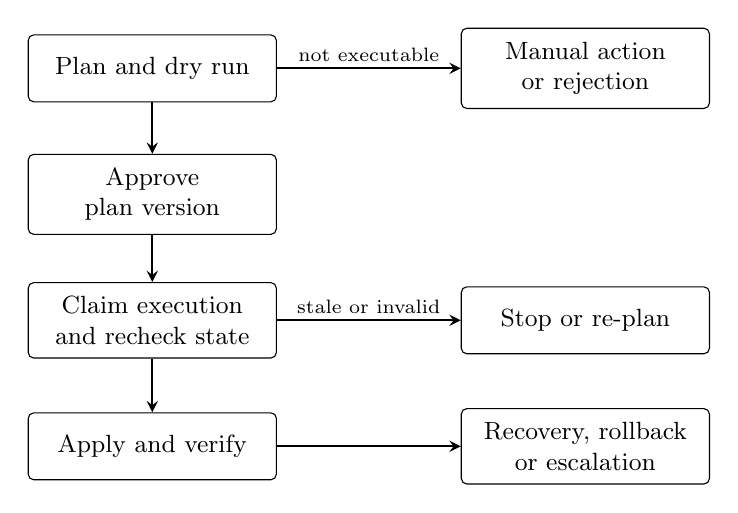
\begin{tikzpicture}[
  box/.style={draw, rounded corners=2pt, align=center, font=\small,
              text width=2.8cm, minimum height=0.85cm, inner sep=5pt},
  flow/.style={->, >=stealth, thick},
  note/.style={font=\scriptsize, fill=white, inner sep=2pt, align=center}]
\node[box] (plan) at (0,0) {Plan and dry run};
\node[box] (approve) at (0,-1.6) {Approve plan version};
\node[box] (recheck) at (0,-3.2) {Claim execution\\and recheck state};
\node[box] (apply) at (0,-4.8) {Apply and verify};
\node[box] (stop) at (5.5,0) {Manual action\\or rejection};
\node[box] (stale) at (5.5,-3.2) {Stop or re-plan};
\node[box] (outcome) at (5.5,-4.8) {Recovery, rollback\\or escalation};
\draw[flow] (plan) -- (approve);
\draw[flow] (plan) -- node[note, above] {not executable} (stop);
\draw[flow] (approve) -- (recheck);
\draw[flow] (recheck) -- (apply);
\draw[flow] (recheck) -- node[note, above] {stale or invalid} (stale);
\draw[flow] (apply) -- (outcome);
\end{tikzpicture}
\caption{Remediation workflow. Rejection or expiry prevents execution.
Re-planning creates a new version requiring new approval. Recovery and
rollback are independently verified outcomes.}
\label{fig:design:approval}
\end{figure}

The executor has its own identity with write permissions limited to the
authorised test resources. The investigation host has read permissions
for operational sources and cannot obtain that identity's credentials.
The executor reads the durable approval and plan, validates their match,
and claims the execution using a conditional state update. Repeated clicks
or delivery of the same request refer to the same execution identifier
and cannot start another copy.

Before changing a resource, the executor serialises actions for that
target, re-reads its state and checks the recorded preconditions. A stale
state comparison requires a new plan or renewed validation and approval.
The execution intent and rollback material must be durably stored before
the write begins. If that storage operation fails, no change is attempted.
This is a stronger requirement than best-effort diagnostic logging.

The resource update and the investigation record are not one atomic
transaction. A timeout can therefore leave the change outcome unknown.
The executor does not blindly retry a potentially completed mutation.
It queries the target and provider operation status to reconcile the
result. If it cannot establish the outcome, it blocks further automated
changes to that target and escalates. Resource-level conditional writes
are used where available, and their absence is recorded as a limit on
protection against concurrent external changes.

\subsection{Recovery and Rollback}

Execution success means that the requested management operation completed.
Recovery requires a legitimate request through the investigated hostname
and operation, together with the plan's relevant state and telemetry
checks. A healthy generic probe does not establish recovery of a failing
authenticated operation. The verifier records observed responses and
their times across the observation period fixed by the evaluation
protocol. The existing 240-second platform health-probe interval remains
separate from these explicit verification requests.

The plan defines whether a failed verification permits an already approved
rollback or requires an operator decision. The interface also provides
an authorised rollback action for an eligible completed change. The
executor verifies that the current state is compatible with restoration
before applying it, preventing a later unrelated change from being
silently overwritten. Restoring the captured configuration and restoring
healthy service have separate outcomes. If the pre-repair configuration
contained the injected fault, a correct rollback may restore that fault.
Returning the experiment to its healthy initial state is then the fault
harness's responsibility, not a successful-recovery claim.

For actions governed by infrastructure code, a pull request is a proposed
change rather than an executed repair. Recovery can only be assessed
after the authorised deployment has applied it. Direct changes to test
resources also need an explicit relationship to their declared
configuration so that a subsequent deployment does not silently undo the
repair. The action policy records that relationship for each supported
adapter.

\section{Operator Interface and Investigation History}
\label{sec:design:interface}

The PoC interface provides a small set of controls: send a test request,
start an investigation, inspect its evidence and review a repair. The
request button invokes a bounded request sender in the investigation host.
It uses a configured Cloudflare-facing hostname and approved operation,
with any necessary test identity. It does not send production telemetry
into the test API. Its purpose is to produce observable application
behaviour through the path being investigated.

The sender records the request time, duration, response status and
available correlation headers. Its endpoint catalogue prevents arbitrary
URL submission, and redirects outside the allowed target are rejected.
Both the sender's network route and its access configuration must permit
the Cloudflare-facing request. Direct calls to an internal application
address are a different check and are labelled separately. The same
request contract supports automated workloads and recovery checks.

The result view shows the primary conclusion, component, cause and
uncertainty before the detailed evidence. Selecting a claim opens the
retained records that support it. A path view distinguishes observed and
inferred links and leaves gaps visible. Query failures and missing source
coverage have their own indicators, so that an empty panel cannot be
mistaken for evidence of health. The plan view shows the target, before
and proposed state, dry-run limits and recovery and rollback conditions
before exposing approval controls.

Entra ID authentication is checked by the backend. Viewing investigations
and starting permitted checks requires the viewing permission. Approval
and rollback require the separate approver permission. Hiding a button
is only an interface convenience and does not authorise an action.
History records retain the diagnosis, plan versions, decisions and each
execution, recovery and rollback outcome. A later investigation creates
a new record instead of overwriting the evidence behind an earlier
decision. The interface has no dependency on the availability of the
test API's own web pages.

\section{Support for Controlled Evaluation}
\label{sec:design:evaluation}

The fault harness is an external experimental component. It prepares and
resets authorised system conditions and records the known cause in the
reference store. It does not expose an injection tool to the investigator.
Development controls and final-case controls use separate permissions,
with the reserved reference record available only to the case custodian
until outputs have been fixed. Test requests use ordinary operational
paths and identifiers. Fault names must not appear in agent-visible logs,
resource labels or symptom descriptions as an answer shortcut.

The evaluation runner creates a fresh investigation for each scheduled
method and repetition. A run manifest identifies the evidence collection
and view, code revision, strategy, prompts or rule versions, model
configuration and limits. Configuration changes produce a different
manifest. The runner records the schedule and termination reason, then
exports the common result fields for scoring. Method labels can be
removed from the review export without removing evidence references.

Live connector checks establish that records can be retrieved and scoped.
The retained-evidence adapter establishes a stable diagnostic comparison,
while the executor and request sender support separate live recovery
tests. These are different execution modes with explicit records, rather
than one demonstration from which every claim is inferred. The resulting
design makes evidence access, diagnostic organisation and authority to
change the test environment independently inspectable.
